\section{Evaluación, comparación de modelos y resultados}
\label{sec:evaluacion}

\subsection{Resultados experimentales}
\label{sec:resultados_exp}

Para cada una de las tres fuentes de datos disponibles (\texttt{sourceId} = 1, 2 y 5), se ha seleccionado el mejor modelo entrenado para cada una de las dos arquitecturas evaluadas: \texttt{MLP} y \texttt{Trafficformer}. La selección se ha realizado tomando como criterio el valor mínimo de la métrica de pérdida sobre el conjunto de validación (\texttt{val\_loss}) entre todas las combinaciones de hiperparámetros evaluadas durante el proceso experimental.

En el \hyperref[anexo:resultados_exp]{Anexo~G} se puede consultar la tabla completa de todos los experimentos llevados a cabo junto con los resultados de todas las métricas obtenidas.

En la tabla~\ref{tab:mejores_modelos} se muestran los modelos seleccionados junto con sus respectivas métricas sobre el conjunto de test, así como los valores clave de los hiperparámetros empleados.

\begin{table}[H]
	\centering
	\small
	\caption{Resultados de los mejores modelos por combinación \texttt{sourceId}--arquitectura}
	\label{tab:mejores_modelos}
	\begin{tabularx}{\textwidth}{c | c | c | c | c | c | c | c }
		\toprule
		\textbf{SID} & \textbf{M} & \textbf{EP} & \textbf{TL} & \textbf{TMAE} & \textbf{TRMSE} & \textbf{TMAPE} & \textbf{TR2} \\
		\midrule
		1 & mlp           & 67 & 0.000 & 25.466 & 38.489   & 1.853   & 0.759 \\
		1 & trafficformer & 30 & 0.143 & 19.125 & 30.784   & 1.745   & 0.822 \\
		2 & mlp           & 30 & 0.000 & 31.017 & 38.177   & 1.82e14 & 0.866 \\
		2 & trafficformer & 96 & 0.002 & 5.832  & 15.046   & 1.51e3  & 0.982 \\
		5 & mlp           & 39 & 0.000 & 213.850 & 343.603 & 4.83e5  & -1.797 \\
		5 & trafficformer & 29 & 0.153 & 175.975 & 306.134 & 1.74e5  & 0.640 \\
		\bottomrule
	\end{tabularx}
	\vspace{0.5em}
	\begin{minipage}{0.98\textwidth}
	\footnotesize
	\textbf{Leyenda de columnas:} \\
	\textbf{SID}: sourceId. \\
	\textbf{M}: Modelo. \\
	\textbf{EP}: Epoch óptima. \\
	\textbf{TL}: Test Loss. \\
	\textbf{TMAE}: Test MAE. \\
	\textbf{TRMSE}: Test RMSE. \\
	\textbf{TMAPE}: Test MAPE. \\
	\textbf{TR2}: Test $R^2$. \\
	Los valores muy grandes se muestran en notación científica (\texttt{a.eb} significa $a \times 10^{b}$). Decimales reducidos para mejorar la presentación.
	\end{minipage}
\end{table}

%%

A continuación se muestran, para cada una de las combinaciones óptimas de fuente de datos (\texttt{sourceId}) y arquitectura (\texttt{MLP} y \texttt{Trafficformer}), las curvas de evolución de las principales métricas durante el entrenamiento. Estas gráficas permiten visualizar el comportamiento del proceso de aprendizaje en términos de error (loss), precisión (MAE, MAPE, MSE, RMSE), y capacidad explicativa ($R^2$), tanto en entrenamiento como en validación. De este modo, se facilita la identificación de fenómenos de sobreajuste, convergencia y diferencias entre arquitecturas y datasets.

Cada figura agrupa, en formato compacto, las seis métricas principales para cada modelo, mostrando la evolución época a época.

\begin{figure}[H]
	\centering
	\begin{minipage}{0.48\textwidth}
		\centering
		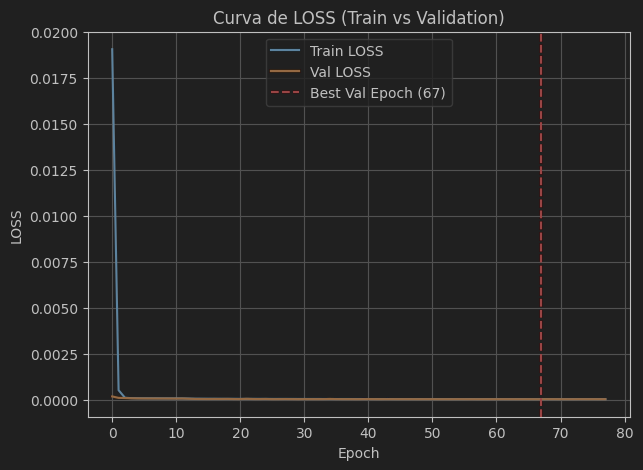
\includegraphics[width=\linewidth]{includes/cap5/graphs/sid1_mlp_loss.png}
		\subcaption{Loss}
		\vspace{0.2cm}
		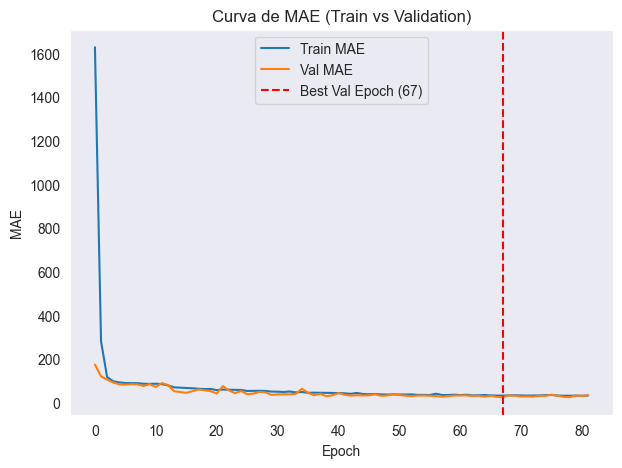
\includegraphics[width=\linewidth]{includes/cap5/graphs/sid1_mlp_mae.png}
		\subcaption{MAE}
		\vspace{0.2cm}
		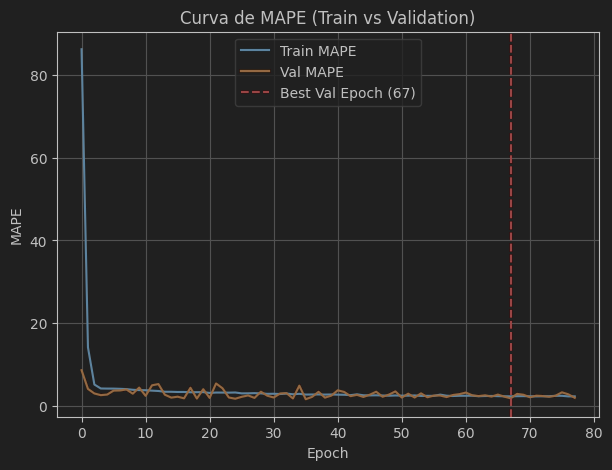
\includegraphics[width=\linewidth]{includes/cap5/graphs/sid1_mlp_mape.png}
		\subcaption{MAPE}
	\end{minipage}
	\hfill
	\begin{minipage}{0.48\textwidth}
		\centering
		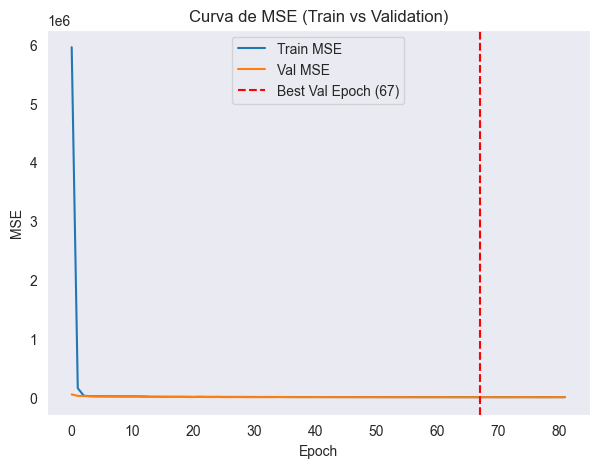
\includegraphics[width=\linewidth]{includes/cap5/graphs/sid1_mlp_mse.png}
		\subcaption{MSE}
		\vspace{0.2cm}
		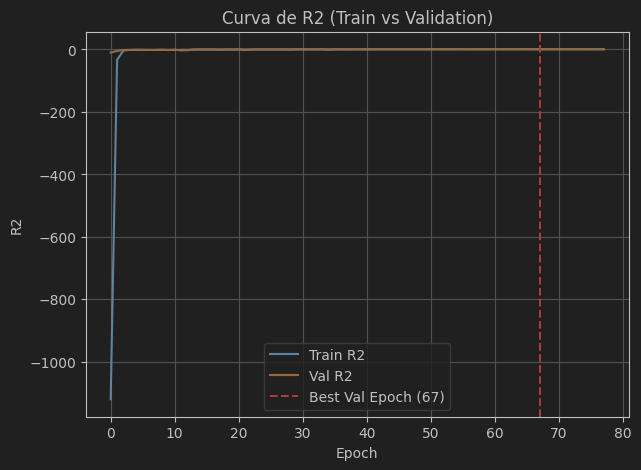
\includegraphics[width=\linewidth]{includes/cap5/graphs/sid1_mlp_r2.png}
		\subcaption{$R^2$}
		\vspace{0.2cm}
		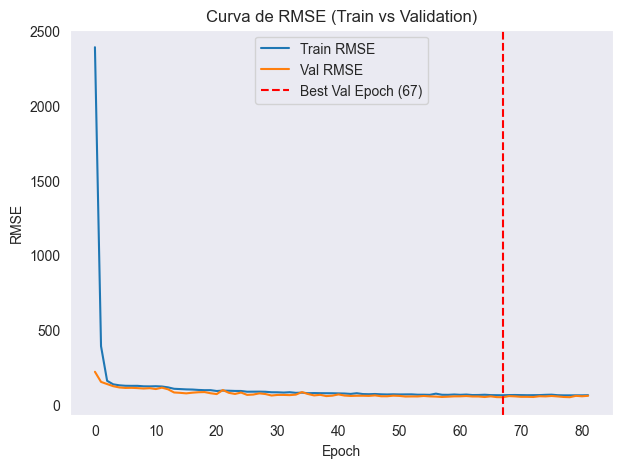
\includegraphics[width=\linewidth]{includes/cap5/graphs/sid1_mlp_rmse.png}
		\subcaption{RMSE}
	\end{minipage}
	\caption{Curvas de entrenamiento para el modelo \texttt{MLP} con datos del Gobierno Vasco (sourceId 1).}
	\label{fig:curvas_sid1_mlp}
\end{figure}

\begin{figure}[H]
	\centering
	\begin{minipage}{0.48\textwidth}
		\centering
		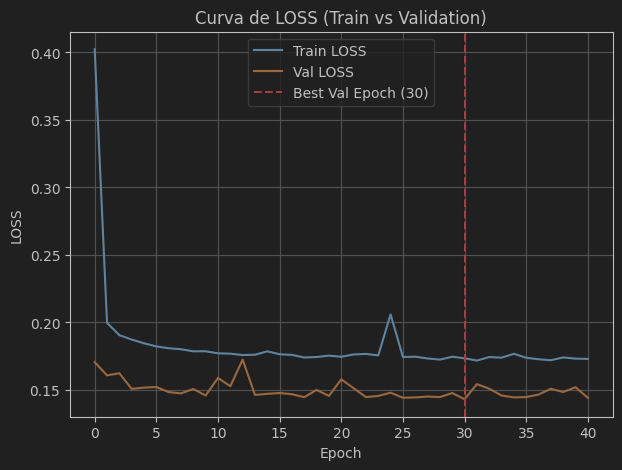
\includegraphics[width=\linewidth]{includes/cap5/graphs/sid1_trafficformer_loss.png}
		\subcaption{Loss}
		\vspace{0.2cm}
		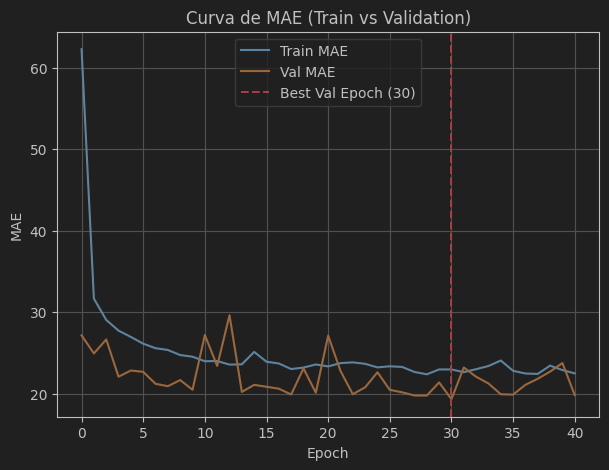
\includegraphics[width=\linewidth]{includes/cap5/graphs/sid1_trafficformer_mae.png}
		\subcaption{MAE}
		\vspace{0.2cm}
		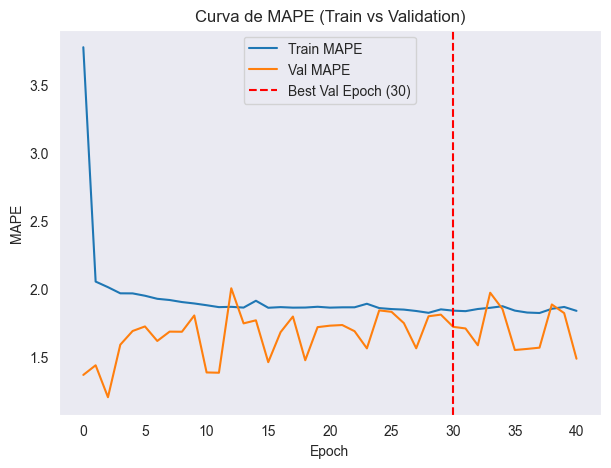
\includegraphics[width=\linewidth]{includes/cap5/graphs/sid1_trafficformer_mape.png}
		\subcaption{MAPE}
	\end{minipage}
	\hfill
	\begin{minipage}{0.48\textwidth}
		\centering
		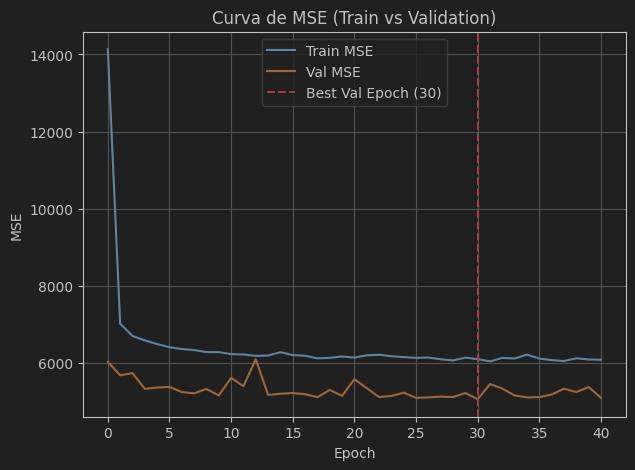
\includegraphics[width=\linewidth]{includes/cap5/graphs/sid1_trafficformer_mse.png}
		\subcaption{MSE}
		\vspace{0.2cm}
		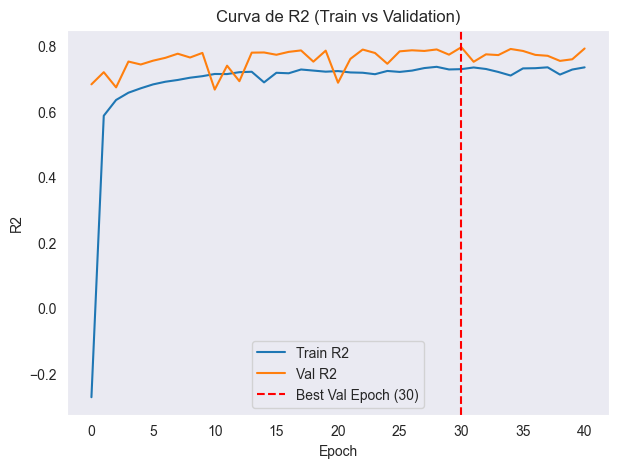
\includegraphics[width=\linewidth]{includes/cap5/graphs/sid1_trafficformer_r2.png}
		\subcaption{$R^2$}
		\vspace{0.2cm}
		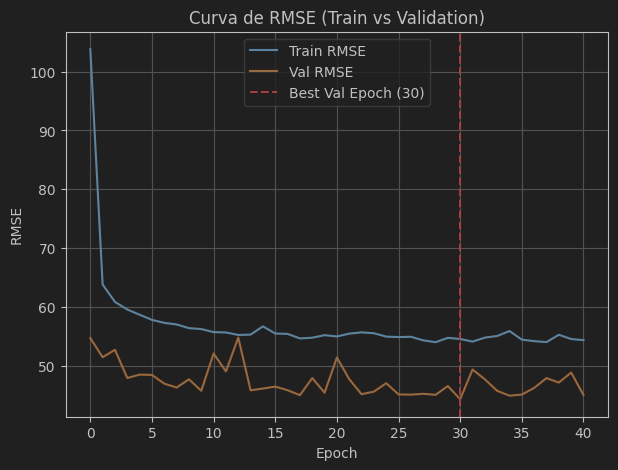
\includegraphics[width=\linewidth]{includes/cap5/graphs/sid1_trafficformer_rmse.png}
		\subcaption{RMSE}
	\end{minipage}
	\caption{Curvas de entrenamiento para el modelo \texttt{Trafficformer} con datos del Gobierno Vasco (sourceId 1).}
	\label{fig:curvas_sid1_trafficformer}
\end{figure}

%%

\begin{figure}[H]
	\centering
	\begin{minipage}{0.48\textwidth}
		\centering
		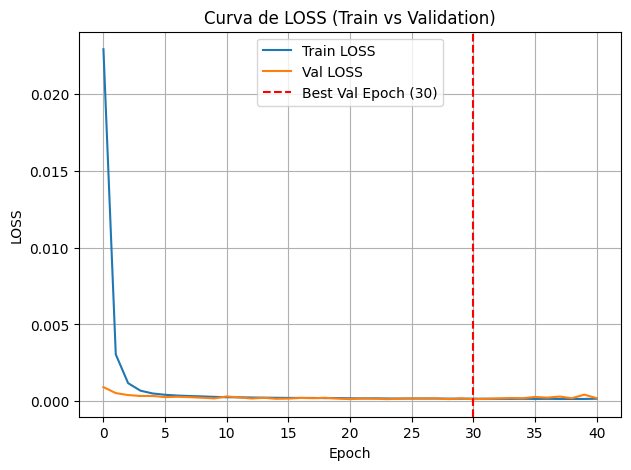
\includegraphics[width=\linewidth]{includes/cap5/graphs/sid2_mlp_loss.png}
		\subcaption{Loss}
		\vspace{0.2cm}
		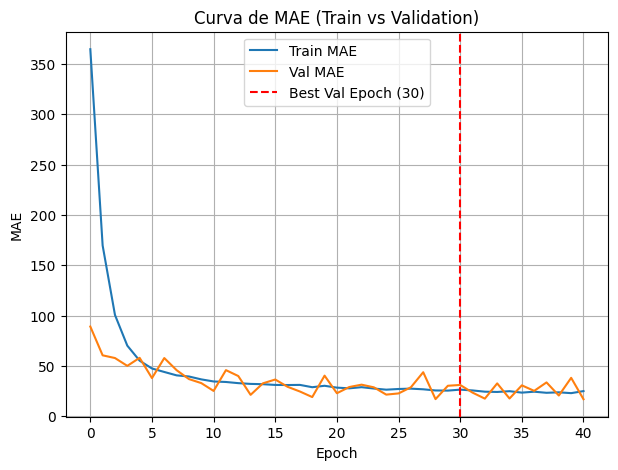
\includegraphics[width=\linewidth]{includes/cap5/graphs/sid2_mlp_mae.png}
		\subcaption{MAE}
		\vspace{0.2cm}
		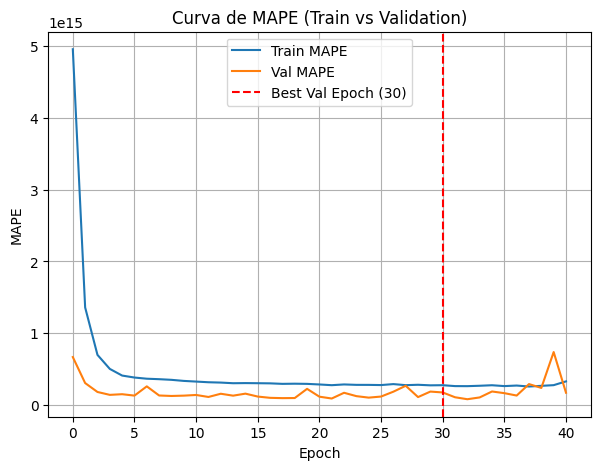
\includegraphics[width=\linewidth]{includes/cap5/graphs/sid2_mlp_mape.png}
		\subcaption{MAPE}
	\end{minipage}
	\hfill
	\begin{minipage}{0.48\textwidth}
		\centering
		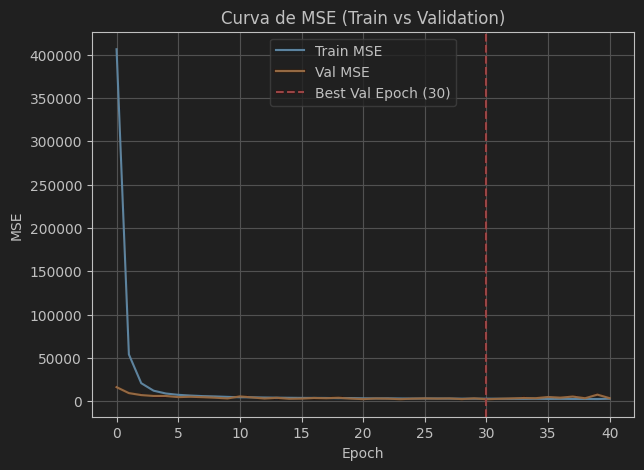
\includegraphics[width=\linewidth]{includes/cap5/graphs/sid2_mlp_mse.png}
		\subcaption{MSE}
		\vspace{0.2cm}
		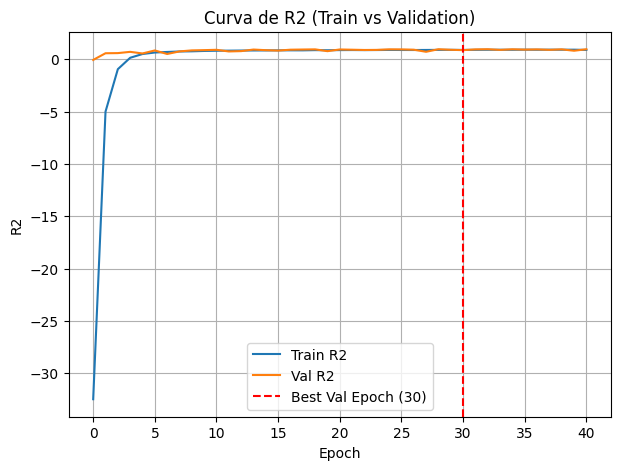
\includegraphics[width=\linewidth]{includes/cap5/graphs/sid2_mlp_r2.png}
		\subcaption{$R^2$}
		\vspace{0.2cm}
		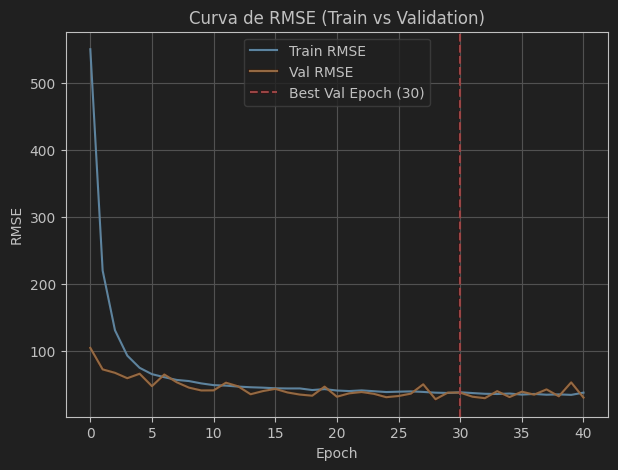
\includegraphics[width=\linewidth]{includes/cap5/graphs/sid2_mlp_rmse.png}
		\subcaption{RMSE}
	\end{minipage}
	\caption{Curvas de entrenamiento para el modelo \texttt{MLP} con datos de la Diputación Foral de Bizkaia (sourceId 2).}
	\label{fig:curvas_sid2_mlp}
\end{figure}

\begin{figure}[H]
	\centering
	\begin{minipage}{0.48\textwidth}
		\centering
		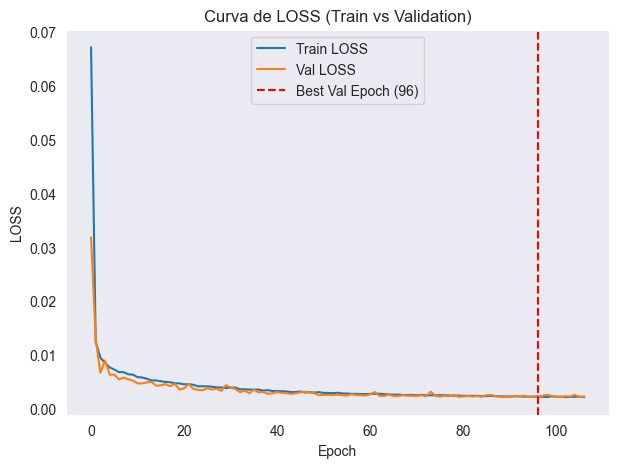
\includegraphics[width=\linewidth]{includes/cap5/graphs/sid2_trafficformer_loss.png}
		\subcaption{Loss}
		\vspace{0.2cm}
		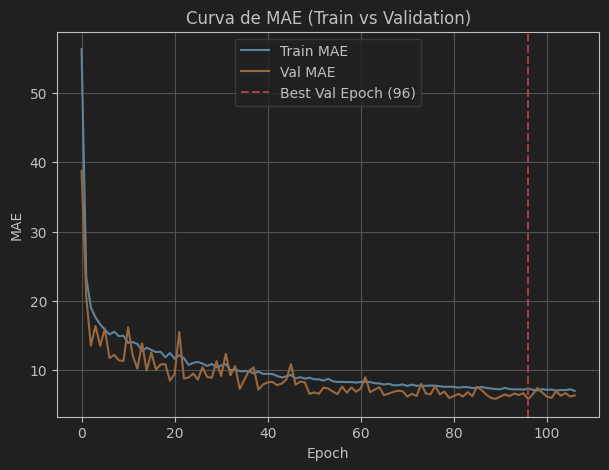
\includegraphics[width=\linewidth]{includes/cap5/graphs/sid2_trafficformer_mae.png}
		\subcaption{MAE}
		\vspace{0.2cm}
		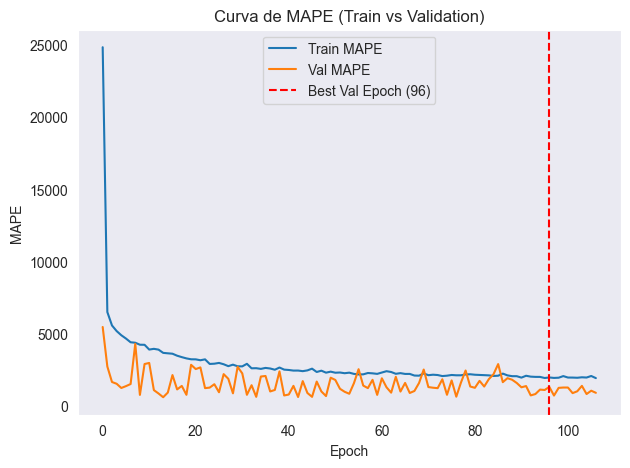
\includegraphics[width=\linewidth]{includes/cap5/graphs/sid2_trafficformer_mape.png}
		\subcaption{MAPE}
	\end{minipage}
	\hfill
	\begin{minipage}{0.48\textwidth}
		\centering
		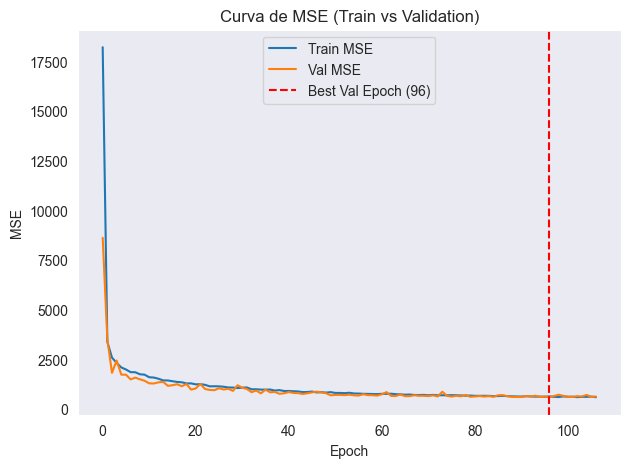
\includegraphics[width=\linewidth]{includes/cap5/graphs/sid2_trafficformer_mse.png}
		\subcaption{MSE}
		\vspace{0.2cm}
		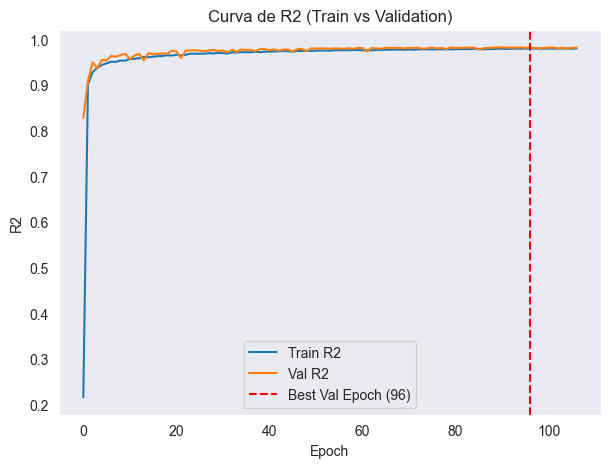
\includegraphics[width=\linewidth]{includes/cap5/graphs/sid2_trafficformer_r2.png}
		\subcaption{$R^2$}
		\vspace{0.2cm}
		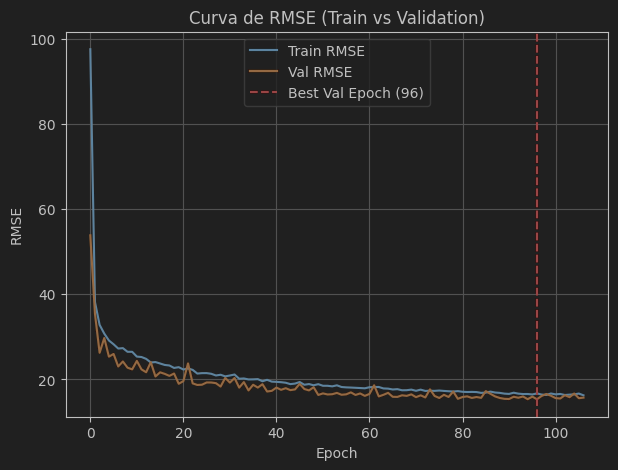
\includegraphics[width=\linewidth]{includes/cap5/graphs/sid2_trafficformer_rmse.png}
		\subcaption{RMSE}
	\end{minipage}
	\caption{Curvas de entrenamiento para el modelo \texttt{Trafficformer} con datos de la Diputación Foral de Bizkaia (sourceId 2).}
	\label{fig:curvas_sid2_trafficformer}
\end{figure}

%%

\begin{figure}[H]
	\centering
	\begin{minipage}{0.48\textwidth}
		\centering
		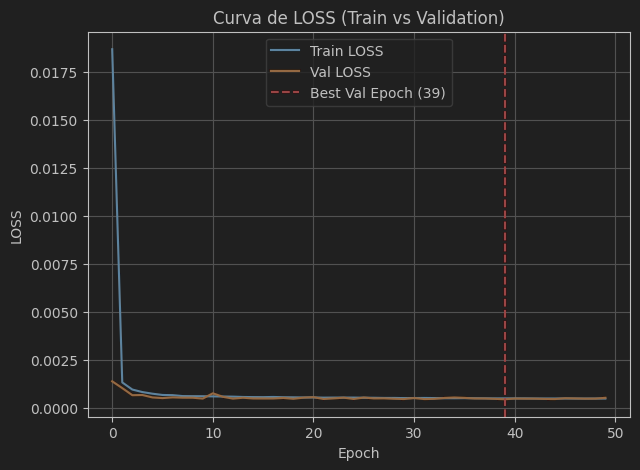
\includegraphics[width=\linewidth]{includes/cap5/graphs/sid5_mlp_loss.png}
		\subcaption{Loss}
		\vspace{0.2cm}
		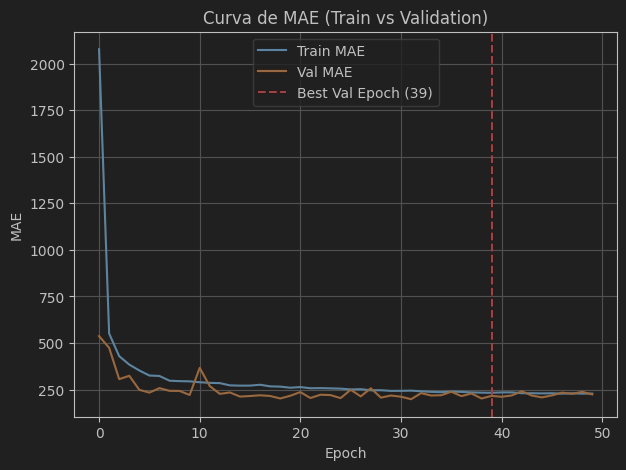
\includegraphics[width=\linewidth]{includes/cap5/graphs/sid5_mlp_mae.png}
		\subcaption{MAE}
		\vspace{0.2cm}
		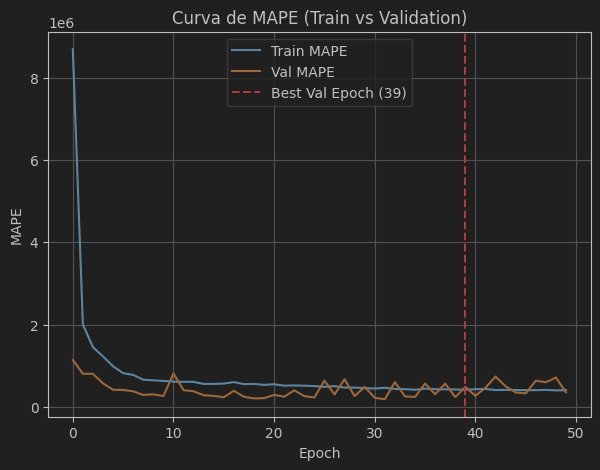
\includegraphics[width=\linewidth]{includes/cap5/graphs/sid5_mlp_mape.png}
		\subcaption{MAPE}
	\end{minipage}
	\hfill
	\begin{minipage}{0.48\textwidth}
		\centering
		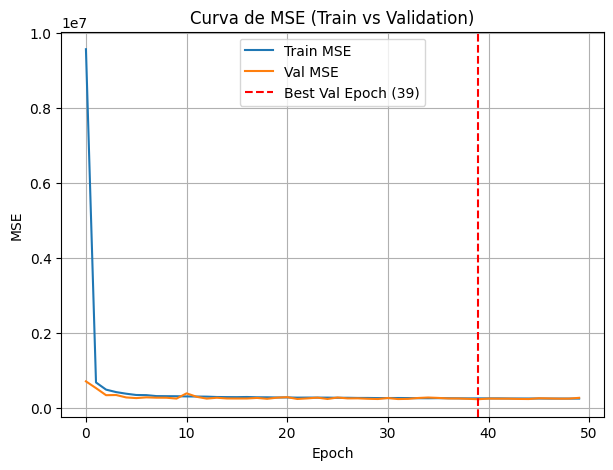
\includegraphics[width=\linewidth]{includes/cap5/graphs/sid5_mlp_mse.png}
		\subcaption{MSE}
		\vspace{0.2cm}
		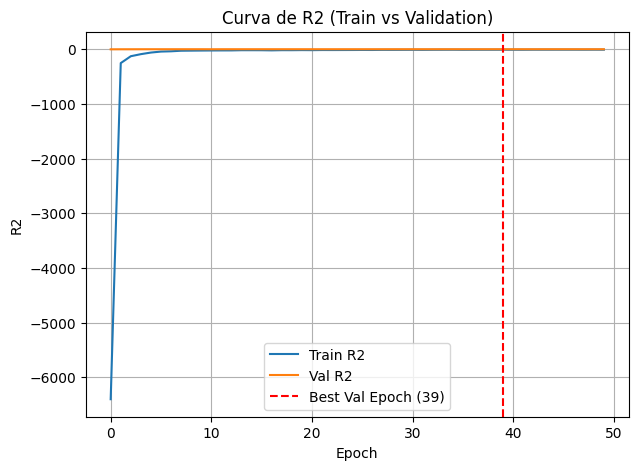
\includegraphics[width=\linewidth]{includes/cap5/graphs/sid5_mlp_r2.png}
		\subcaption{$R^2$}
		\vspace{0.2cm}
		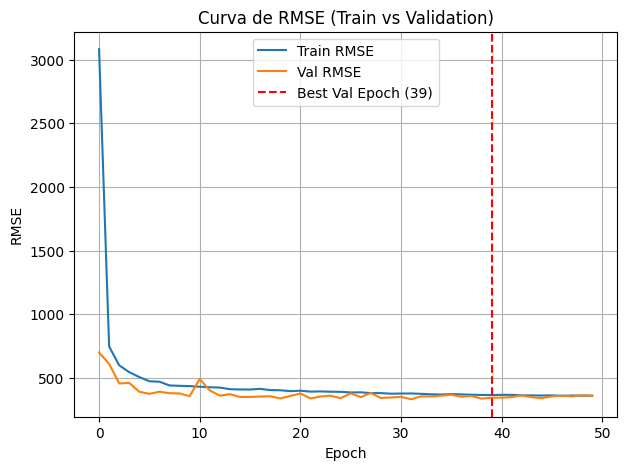
\includegraphics[width=\linewidth]{includes/cap5/graphs/sid5_mlp_rmse.png}
		\subcaption{RMSE}
	\end{minipage}
	\caption{Curvas de entrenamiento para el modelo \texttt{MLP} con datos del Ayuntamiento de Bilbao (sourceId 5).}
	\label{fig:curvas_sid5_mlp}
\end{figure}

\begin{figure}[H]
	\centering
	\begin{minipage}{0.48\textwidth}
		\centering
		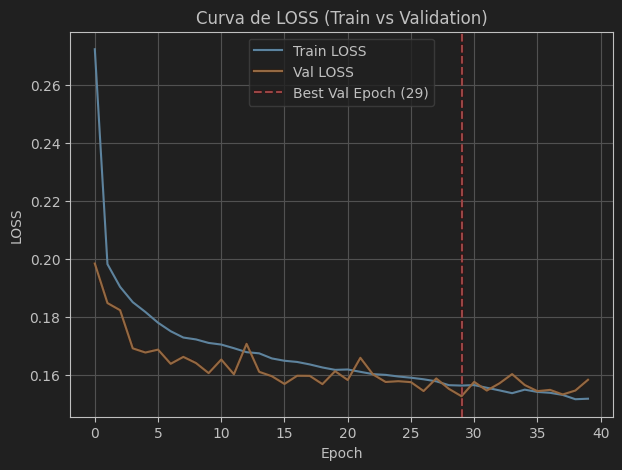
\includegraphics[width=\linewidth]{includes/cap5/graphs/sid5_trafficformer_loss.png}
		\subcaption{Loss}
		\vspace{0.2cm}
		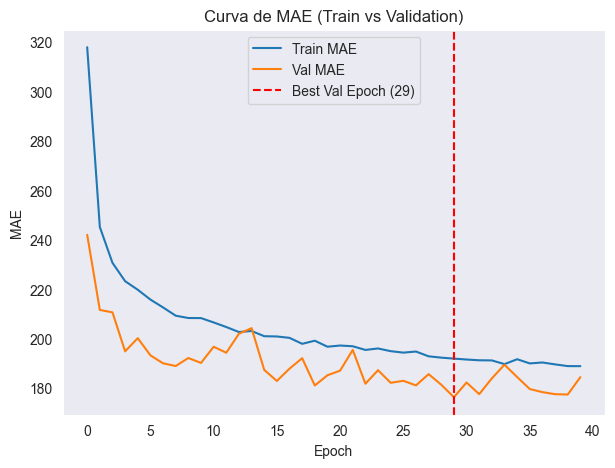
\includegraphics[width=\linewidth]{includes/cap5/graphs/sid5_trafficformer_mae.png}
		\subcaption{MAE}
		\vspace{0.2cm}
		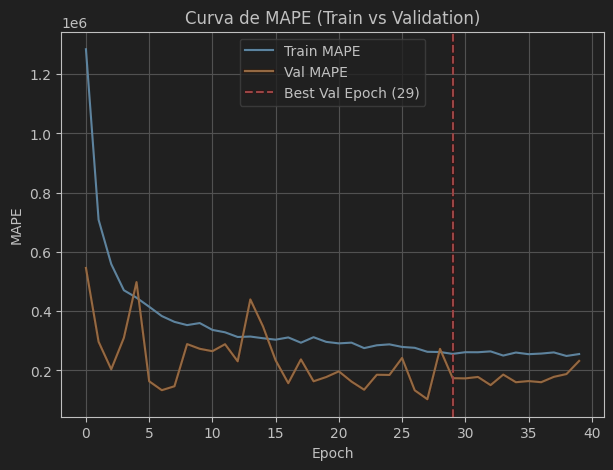
\includegraphics[width=\linewidth]{includes/cap5/graphs/sid5_trafficformer_mape.png}
		\subcaption{MAPE}
	\end{minipage}
	\hfill
	\begin{minipage}{0.48\textwidth}
		\centering
		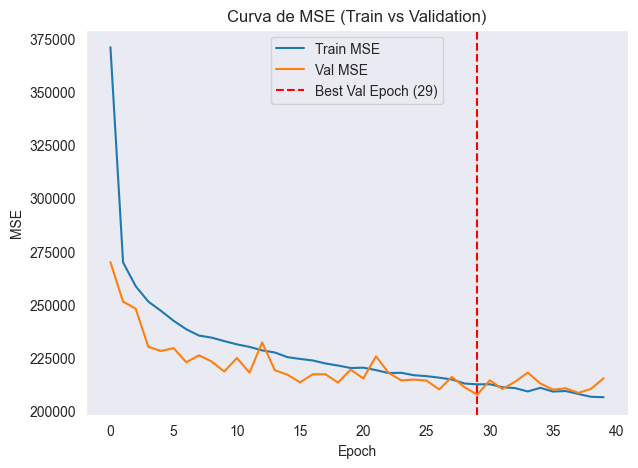
\includegraphics[width=\linewidth]{includes/cap5/graphs/sid5_trafficformer_mse.png}
		\subcaption{MSE}
		\vspace{0.2cm}
		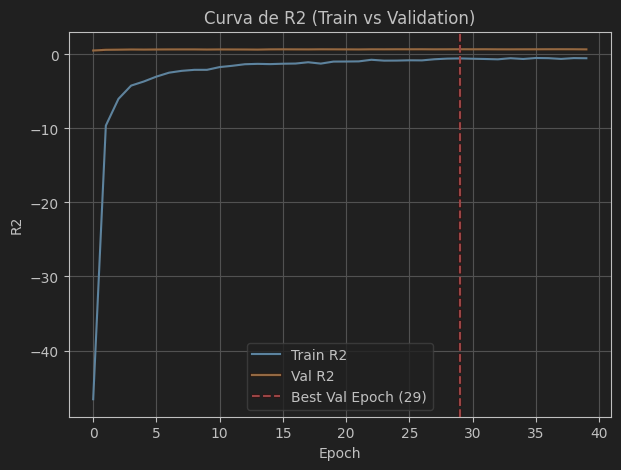
\includegraphics[width=\linewidth]{includes/cap5/graphs/sid5_trafficformer_r2.png}
		\subcaption{$R^2$}
		\vspace{0.2cm}
		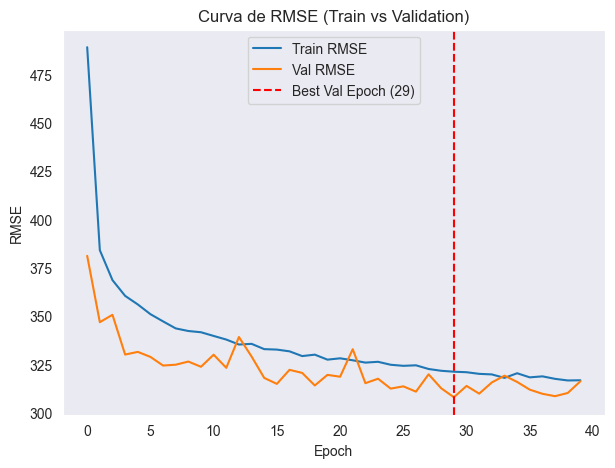
\includegraphics[width=\linewidth]{includes/cap5/graphs/sid5_trafficformer_rmse.png}
		\subcaption{RMSE}
	\end{minipage}
	\caption{Curvas de entrenamiento para el modelo \texttt{Trafficformer} con datos del Ayuntamiento de Bilbao (sourceId 5).}
	\label{fig:curvas_sid5_trafficformer}
\end{figure}

Antes de analizar en profundidad los resultados, conviene contextualizar los experimentos realizados respecto al modelo original Trafficformer propuesto por \cite{trafficformer}. En dicho estudio, la evaluación se realizó sobre el \textit{Seattle Loop Detector Dataset}, un conjunto de datos altamente estructurado y representativo de una red viaria en anillo con características propias, tanto en topología como en calidad de señal.

Por el contrario, en el presente trabajo se han utilizado datos abiertos de diferentes fuentes públicas, correspondientes a la provincia de Bizkaia y el entorno urbano de Bilbao, incluyendo sensores instalados en redes viarias de distinta naturaleza (autonómica, foral y municipal) y sometidos a procesos adicionales de integración, limpieza y preprocesamiento. Esta heterogeneidad y variabilidad inherente a los datos introduce desafíos adicionales en el modelado y la predicción.

A pesar de estas diferencias, los resultados obtenidos son comparables en términos de magnitud y tendencia a los reportados por Chang et al., lo que evidencia la solidez y capacidad de generalización de la arquitectura Trafficformer, incluso en contextos con fuentes de datos abiertas, distribuidas y heterogéneas. Esta comparativa refuerza la validez de las conclusiones presentadas a continuación y pone en valor la adaptabilidad del modelo a diferentes escenarios reales de predicción de tráfico.

Todas las curvas y métricas detalladas para los 120 experimentos están disponibles en la plataforma \textit{Weights \& Biases}.

%%

\subsection{Discusión y análisis crítico}
\label{sec:discusion_analisis}

\begin{comment}
	- Interpretación de los resultados:
	- ¿Dónde y por qué Trafficformer supera a MLP?
	- ¿Hay algún caso donde no sea así?
	- Relación con lo observado en el estado del arte.
	- Reflexión sobre la influencia de los hiperparámetros, la ventana temporal y el tamaño del batch.
\end{comment}

En esta sección se realiza una evaluación crítica y comparativa de los resultados obtenidos por las dos arquitecturas propuestas (MLP y Trafficformer), para cada una de las tres fuentes de datos analizadas (sourceIds 1, 2 y 5). Se emplean las métricas reportadas en la tabla~\ref{tab:mejores_modelos}, junto con las gráficas de entrenamiento para cada modelo, para ofrecer un análisis detallado sobre la superioridad y limitaciones observadas.

\subsubsection*{Comparativa en datos del Gobierno Vasco (sourceId 1)}

El conjunto de datos del Gobierno Vasco incluye un total de 386 sensores (\textit{meters}), aunque estos se encuentran ubicados en unos pocos puntos estratégicos distribuidos linealmente a lo largo de vías principales, como se observa en la Figura~\ref{fig:sensores_sid1} (véase capítulo anterior). Cada sensor representa un carril individual, lo que genera una alta densidad espacial en áreas críticas, pero una baja dispersión geográfica global. El dataset empleado para el entrenamiento tiene una dimensionalidad de entrada de 14\,828 ventanas temporales, con una longitud de secuencia (\texttt{seq\_len}) de 8 (equivalente a ventanas de 4 horas). El conjunto de entrenamiento consta de 10\,379 muestras, el de validación de 2\,980 y el de test de 1\,469. Esta configuración temporal amplia permite a los modelos captar patrones dinámicos prolongados, aspecto especialmente favorable para el mecanismo de atención espacial de Trafficformer.

La comparativa entre modelos MLP (figura~\ref{fig:curvas_sid1_mlp}) y Trafficformer (figura~\ref{fig:curvas_sid1_trafficformer}) muestra claramente la superioridad de la arquitectura basada en Transformer. Trafficformer obtiene valores significativamente mejores en las métricas de pérdida (loss), MAE, RMSE y MAPE, así como un mayor coeficiente de determinación ($R^2$). En particular, Trafficformer reduce el MAE de 25.466 a 19.125 y el RMSE de 38.489 a 30.784, lo que refleja una mayor capacidad para capturar las complejidades espaciales y temporales de los datos de tráfico en este entorno.

El análisis visual de las curvas de entrenamiento evidencia una convergencia más rápida y estable para Trafficformer, que alcanza su punto óptimo en la época 30, notablemente antes que el modelo MLP (época 67). Este comportamiento puede atribuirse a la capacidad de atención espacial y aprendizaje secuencial del modelo, que permite explotar eficazmente las relaciones entre sensores cercanos.

La disposición lineal y agrupada de los sensores en puntos estratégicos de la red viaria (véase Figura~\ref{fig:sensores_sid1}) facilita que el modelo Trafficformer aproveche las relaciones espaciales locales, incrementando así su desempeño frente a modelos menos estructurados como el MLP.

\subsubsection*{Comparativa en datos Diputación Foral de Bizkaia (sourceId 2)}

La fuente de datos de la Diputación Foral de Bizkaia presenta una distribución geográfica amplia y diversa, cubriendo exhaustivamente la red viaria de Bizkaia, como se aprecia en la Figura~\ref{fig:sensores_sid2} (véase capítulo anterior). Inicialmente se consideraron 520 sensores, aunque tras el filtrado por ausencia de datos el número efectivo de sensores fue de 462. Esta elevada cantidad y dispersión espacial implica una alta complejidad en términos de relaciones y patrones de tráfico. El conjunto de entrenamiento está compuesto por 12\,292 ventanas temporales, mientras que validación y test contienen 3\,530 y 1\,739 ventanas respectivamente. Para esta fuente se ha empleado una ventana temporal más reducida (\texttt{seq\_len} = 4, equivalentes a ventanas de 2 horas), adaptada a la mayor densidad y complejidad espacial de la red. La máscara espacial generada revela numerosas conexiones entre sensores distantes, lo que beneficia de manera significativa al modelo Trafficformer gracias a su capacidad de capturar relaciones espaciales complejas mediante atención multi-cabeza.

La superioridad del modelo Trafficformer respecto al modelo MLP se acentúa aún más en los datos de la Diputación Foral de Bizkaia. Como se observa en las figuras~\ref{fig:curvas_sid2_mlp} y \ref{fig:curvas_sid2_trafficformer}, Trafficformer reduce considerablemente el MAE desde 31.017 hasta 5.832 y el RMSE desde 38.177 hasta 15.046. El $R^2$ mejora sustancialmente de 0.866 (MLP) a 0.982 (Trafficformer), lo que indica una capacidad notablemente superior para explicar la variabilidad en los datos.

Las curvas de entrenamiento muestran una convergencia estable y continua del modelo Trafficformer hasta la época 96, reflejando una adecuada selección de hiperparámetros que permitió una optimización profunda. El modelo MLP, en cambio, converge rápidamente en la época 30, mostrando potencialmente limitaciones en su capacidad para aprovechar plenamente el volumen y complejidad de los datos disponibles.

La amplia y densa distribución geográfica de los sensores para la Diputación Foral de Bizkaia (véase Figura~\ref{fig:sensores_sid2}) permite al modelo Trafficformer capturar relaciones espaciales complejas, aspecto que el modelo MLP no puede explotar debido a su limitada capacidad para modelar dependencias espaciales.

\subsubsection*{Comparativa en datos Ayuntamiento de Bilbao (sourceId 5)}

El tercer conjunto de datos se caracteriza por una cobertura urbana densa, centrada en la ciudad de Bilbao, como se aprecia en la Figura~\ref{fig:sensores_sid5} (véase capítulo anterior). Aunque inicialmente se disponía de 92 sensores, el filtrado por calidad y disponibilidad redujo el número efectivo a 70. Esta elevada concentración espacial en un entorno urbano genera relaciones altamente correlacionadas y complejas entre sensores, lo que presenta retos específicos para los modelos de predicción de tráfico. El dataset consta de 17\,330 ventanas temporales, de las cuales 12\,131 se utilizaron para entrenamiento, 3\,483 para validación y 1\,716 para test. Al igual que en el caso anterior, se utilizó una ventana temporal de 2 horas (\texttt{seq\_len} = 4), permitiendo al modelo captar de manera eficiente las dinámicas urbanas rápidas propias de la ciudad.

Para la fuente sourceId 5, el modelo Trafficformer sigue mostrando una clara ventaja frente al modelo MLP. Según las figuras~\ref{fig:curvas_sid5_mlp} y \ref{fig:curvas_sid5_trafficformer}, se observa una mejora sustancial en todas las métricas principales. El MAE disminuye de 213.850 a 175.975, y el RMSE de 343.603 a 306.134. El coeficiente de determinación $R^2$ experimenta una mejora especialmente relevante, pasando de un valor negativo e inadecuado de -1.797 (MLP) a un aceptable 0.640 (Trafficformer), lo que indica una mayor capacidad para explicar la variabilidad del tráfico urbano.

Las curvas de entrenamiento muestran que Trafficformer converge rápidamente (época 29), evidenciando que su mecanismo de atención espacial resulta especialmente efectivo en escenarios urbanos densos, donde la interacción entre sensores cercanos es particularmente compleja.

La configuración urbana y la alta densidad espacial de los sensores del Ayuntamiento de Bilbao (véase Figura~\ref{fig:sensores_sid5}) genera una compleja red de interacciones espaciales que favorece notablemente al modelo Trafficformer frente al MLP, que carece de mecanismos específicos para gestionar esta complejidad. Este análisis subraya la importancia de adaptar el diseño experimental y la selección de ventanas temporales a las particularidades de cada conjunto de datos, ya que estas decisiones se reflejan directamente en el rendimiento relativo de los modelos evaluados.

\subsection{Análisis avanzado de resultados por fuente de datos}
\label{sec:analisis_avanzado_resultados}

Además del análisis comparativo entre las arquitecturas y fuentes de datos realizado previamente, se ha llevado a cabo un análisis avanzado, complementario y exhaustivo, con el objetivo de identificar patrones específicos y posibles limitaciones de los modelos entrenados. Este análisis incluye gráficos específicos tales como la representación del error absoluto frente a los valores reales, series temporales comparativas para sensores individuales, mapas de errores y gráficos de distribución del error por sensor.

A continuación, se presentan las conclusiones más relevantes derivadas del análisis avanzado realizado para cada una de las fuentes de datos (\texttt{sourceId}). El detalle completo de las gráficas mencionadas está disponible en el \hyperref[anexo:analisis_avanzado]{Anexo~H}.

\subsubsection*{Gobierno Vasco (SourceId 1)}
El análisis avanzado sobre la fuente de datos 1 muestra una adecuada capacidad predictiva global del modelo Trafficformer. El gráfico de dispersión (scatter plot) revela una fuerte correlación entre los valores predichos y los reales, con la mayoría de puntos cercanos a la diagonal. Sin embargo, el histograma de errores refleja la presencia de errores significativos en ciertas predicciones puntuales, lo que sugiere áreas específicas donde el modelo podría mejorar. El mapa de errores confirma visualmente que la mayoría de errores altos se concentran en puntos geográficos específicos (probablemente zonas críticas de tráfico o intersecciones complejas), lo que podría ser causado por factores no capturados completamente por el modelo.

\subsubsection*{Diputación Foral de Bizkaia (SourceId 2)}
En el caso de la fuente de datos 2, se observa un excelente rendimiento del modelo Trafficformer, especialmente notable en el gráfico de dispersión y el histograma de errores, que muestran una alta concentración alrededor del valor real y errores generalmente bajos. Sin embargo, la distribución espacial del error representada en el mapa destaca algunas ubicaciones específicas con errores ligeramente mayores, posiblemente relacionadas con zonas periféricas o sensores más aislados, donde la densidad de datos disponibles para el entrenamiento fue inferior. Las series temporales para los mejores y peores sensores confirman que los mayores errores ocurren en contextos específicos, probablemente vinculados a eventos atípicos o patrones de tráfico inusuales.

\subsubsection*{Ayuntamiento de Bilbao (SourceId 5)}
Finalmente, la fuente de datos 5, que cubre una zona urbana densa (Bilbao), presenta una complejidad intrínseca mayor. Esto se evidencia en el gráfico de dispersión, donde se observa una mayor dispersión de los puntos respecto a la diagonal ideal, indicando predicciones menos precisas para determinados sensores urbanos. El histograma del error muestra una distribución más amplia, sugiriendo heterogeneidad en la capacidad predictiva del modelo según zonas específicas. La distribución espacial de los errores confirma que áreas urbanas densamente pobladas y congestionadas muestran consistentemente errores más elevados, un aspecto esperado dada la complejidad del tráfico urbano.

Este análisis avanzado permite concluir que, aunque el modelo Trafficformer muestra en general buenos resultados en todas las fuentes de datos, existe un margen significativo de mejora en escenarios específicos y complejos, tales como intersecciones críticas y áreas urbanas densas. Además, pone de manifiesto la importancia del análisis visual detallado para identificar oportunidades específicas de optimización en futuras iteraciones del modelo.

\subsubsection*{Síntesis comparativa respecto al estado del arte}

Con el objetivo de contextualizar los resultados obtenidos en este trabajo, se presenta una comparativa entre las métricas alcanzadas por el modelo Trafficformer sobre los distintos conjuntos de datos locales y las reportadas en el estudio original de \cite{trafficformer}. 

\begin{table}[H]
	\centering
	\small
	\caption{Comparativa de resultados de Trafficformer respecto al estado del arte.}
	\label{tab:comparativa_trafficformer}
	\begin{tabularx}{\textwidth}{>{\raggedright\arraybackslash}X c c c c c c}
		\toprule
		& \textbf{Dataset} & \textbf{Variable Predicha} & \textbf{MAE} & \textbf{MAPE (\%)} & \textbf{RMSE} & \textbf{$R^2$} \\
		\midrule
		\textbf{Trafficformer (Chang et al., 2025)} & Seattle Loop & Velocidad (mph) & 2.10 & 4.70 & 3.08 & -- \\
		\textbf{Trafficformer (TFM, SourceId 1)} & Gobierno Vasco & Capacidad (veh/h) & 19.125 & 1.745 & 30.784 & 0.822 \\
		\textbf{Trafficformer (TFM, SourceId 2)} & DFB & Capacidad (veh/h) & 5.832 & 1.51e3 & 15.046 & 0.982 \\
		\textbf{Trafficformer (TFM, SourceId 5)} & Ayto. Bilbao & Capacidad (veh/h) & 175.975 & 1.74e5 & 306.134 & 0.640 \\
		\bottomrule
	\end{tabularx}
\end{table}

Tal y como se recoge en la Tabla~\ref{tab:comparativa_trafficformer}, se aprecia una consistencia en la tendencia favorable del modelo Trafficformer frente a arquitecturas más simples como MLP, en línea con lo observado en la literatura reciente.
Los resultados no son estrictamente comparables, ya que el modelo original evalúa la predicción de velocidades medias (en mph) sobre el dataset Seattle Loop, mientras que en este TFM se predice la capacidad de tráfico (vehículos/hora) en datasets locales distintos (Gobierno Vasco, DFB y Ayuntamiento de Bilbao).

La superioridad generalizada del modelo Trafficformer sobre MLP en las tres fuentes de datos analizadas se explica principalmente por la capacidad de capturar dependencias espaciales y temporales mediante el mecanismo de atención multi-cabezal. Esta capacidad es especialmente valiosa en contextos urbanos complejos (sourceId 5) y en redes de sensores extensas (sourceId 2), donde las relaciones entre los puntos de medida tienen gran relevancia.

La elección de hiperparámetros, como el tamaño del batch, learning rate, número de cabezas de atención y dimensión de embedding, ha demostrado ser crítica en la optimización de Trafficformer. Los resultados muestran que valores intermedios o altos para \texttt{num\_heads} y \texttt{embedding\_dim} mejoran significativamente el rendimiento, validando lo observado en estudios previos del estado del arte~\cite{trafficformer}.

Finalmente, el análisis pone de manifiesto que el modelo MLP presenta limitaciones inherentes a su arquitectura más simple, especialmente en contextos con fuertes correlaciones espaciales o temporales. El modelo Trafficformer, al incluir mecanismos avanzados de atención, proporciona mayor robustez y capacidad predictiva, alineándose con las tendencias recientes en la literatura científica sobre modelos Transformer aplicados a predicción del tráfico.
